\section{Results}
\subsection{Detection Results}

Table~\ref{tab:detection_results} presents the detection performance of RT-DETR and EAST on the Vietnamese document test set. Precision (P), Recall (R), F1, and Average Precision (AP) are reported at IoU thresholds of 0.50 and 0.75, along with mean AP averaged over thresholds from 0.50 to 0.95.

\begin{table}[ht]
\centering
\scriptsize
\caption[Text line detection results on the Vietnamese document test set]{\textit{Text line detection results on the Vietnamese document test set.}}
\label{tab:detection_results}
\begin{tabular}{lcccccccc}
\hline
\textbf{Model} & \textbf{P@.50} & \textbf{R@.50} & \textbf{F1@.50} & \textbf{P@.75} & \textbf{R@.75} & \textbf{F1@.75} & \textbf{AP@.50} & \textbf{mAP.5:.95} \\
\hline
\textbf{RT-DETR (ours)} & \textbf{0.5175} & \textbf{0.4862} & \textbf{0.5014} & \textbf{0.1936} & \textbf{0.1819} & \textbf{0.1876} & \textbf{0.3846} & \textbf{0.1467} \\
EAST & 0.2608 & 0.0902 & 0.1340 & 0.0407 & 0.0141 & 0.0209 & 0.0329 & 0.0080 \\
\hline
\end{tabular}
\end{table}

The fine-tuned RT-DETR model substantially outperforms EAST across all reported metrics. At IoU threshold 0.50, RT-DETR achieves an F1-score of \textbf{0.501} compared to \textbf{0.134} for EAST, representing a relative improvement of 274\%. The AP@0.50 of 0.385 versus 0.033 for EAST further confirms that this advantage is consistent across confidence threshold operating points and is not attributable to a favorable threshold selection. The performance gap is even more pronounced at the stricter IoU threshold of 0.75, where RT-DETR achieves an F1 of \textbf{0.188} against EAST's \textbf{0.021}, a relative improvement of approximately 795\%, and the mAP@0.5:0.95 of \textbf{0.147} versus \textbf{0.008} further quantifies the overall localization quality advantage across the full threshold range.

These results reveal that EAST, despite being a strong general-purpose text detector, fails to generalize to Vietnamese document layouts without domain-specific adaptation, as its axis-aligned detections systematically underfit rotated text regions and produce low IoU even for correctly localized text lines. The disproportionate improvement at IoU 0.75 confirms that the GWD loss and sine-cosine angle encoding contribute meaningfully to bounding box tightness, which is critical for minimizing background noise in the crops passed to the recognition stage.

To provide a more accessible visual summary of these quantitative differences, Figure~\ref{fig:detection_bar} presents a grouped bar chart comparing RT-DETR and EAST across all reported metrics.

\begin{figure}[htbp]
    \centering
    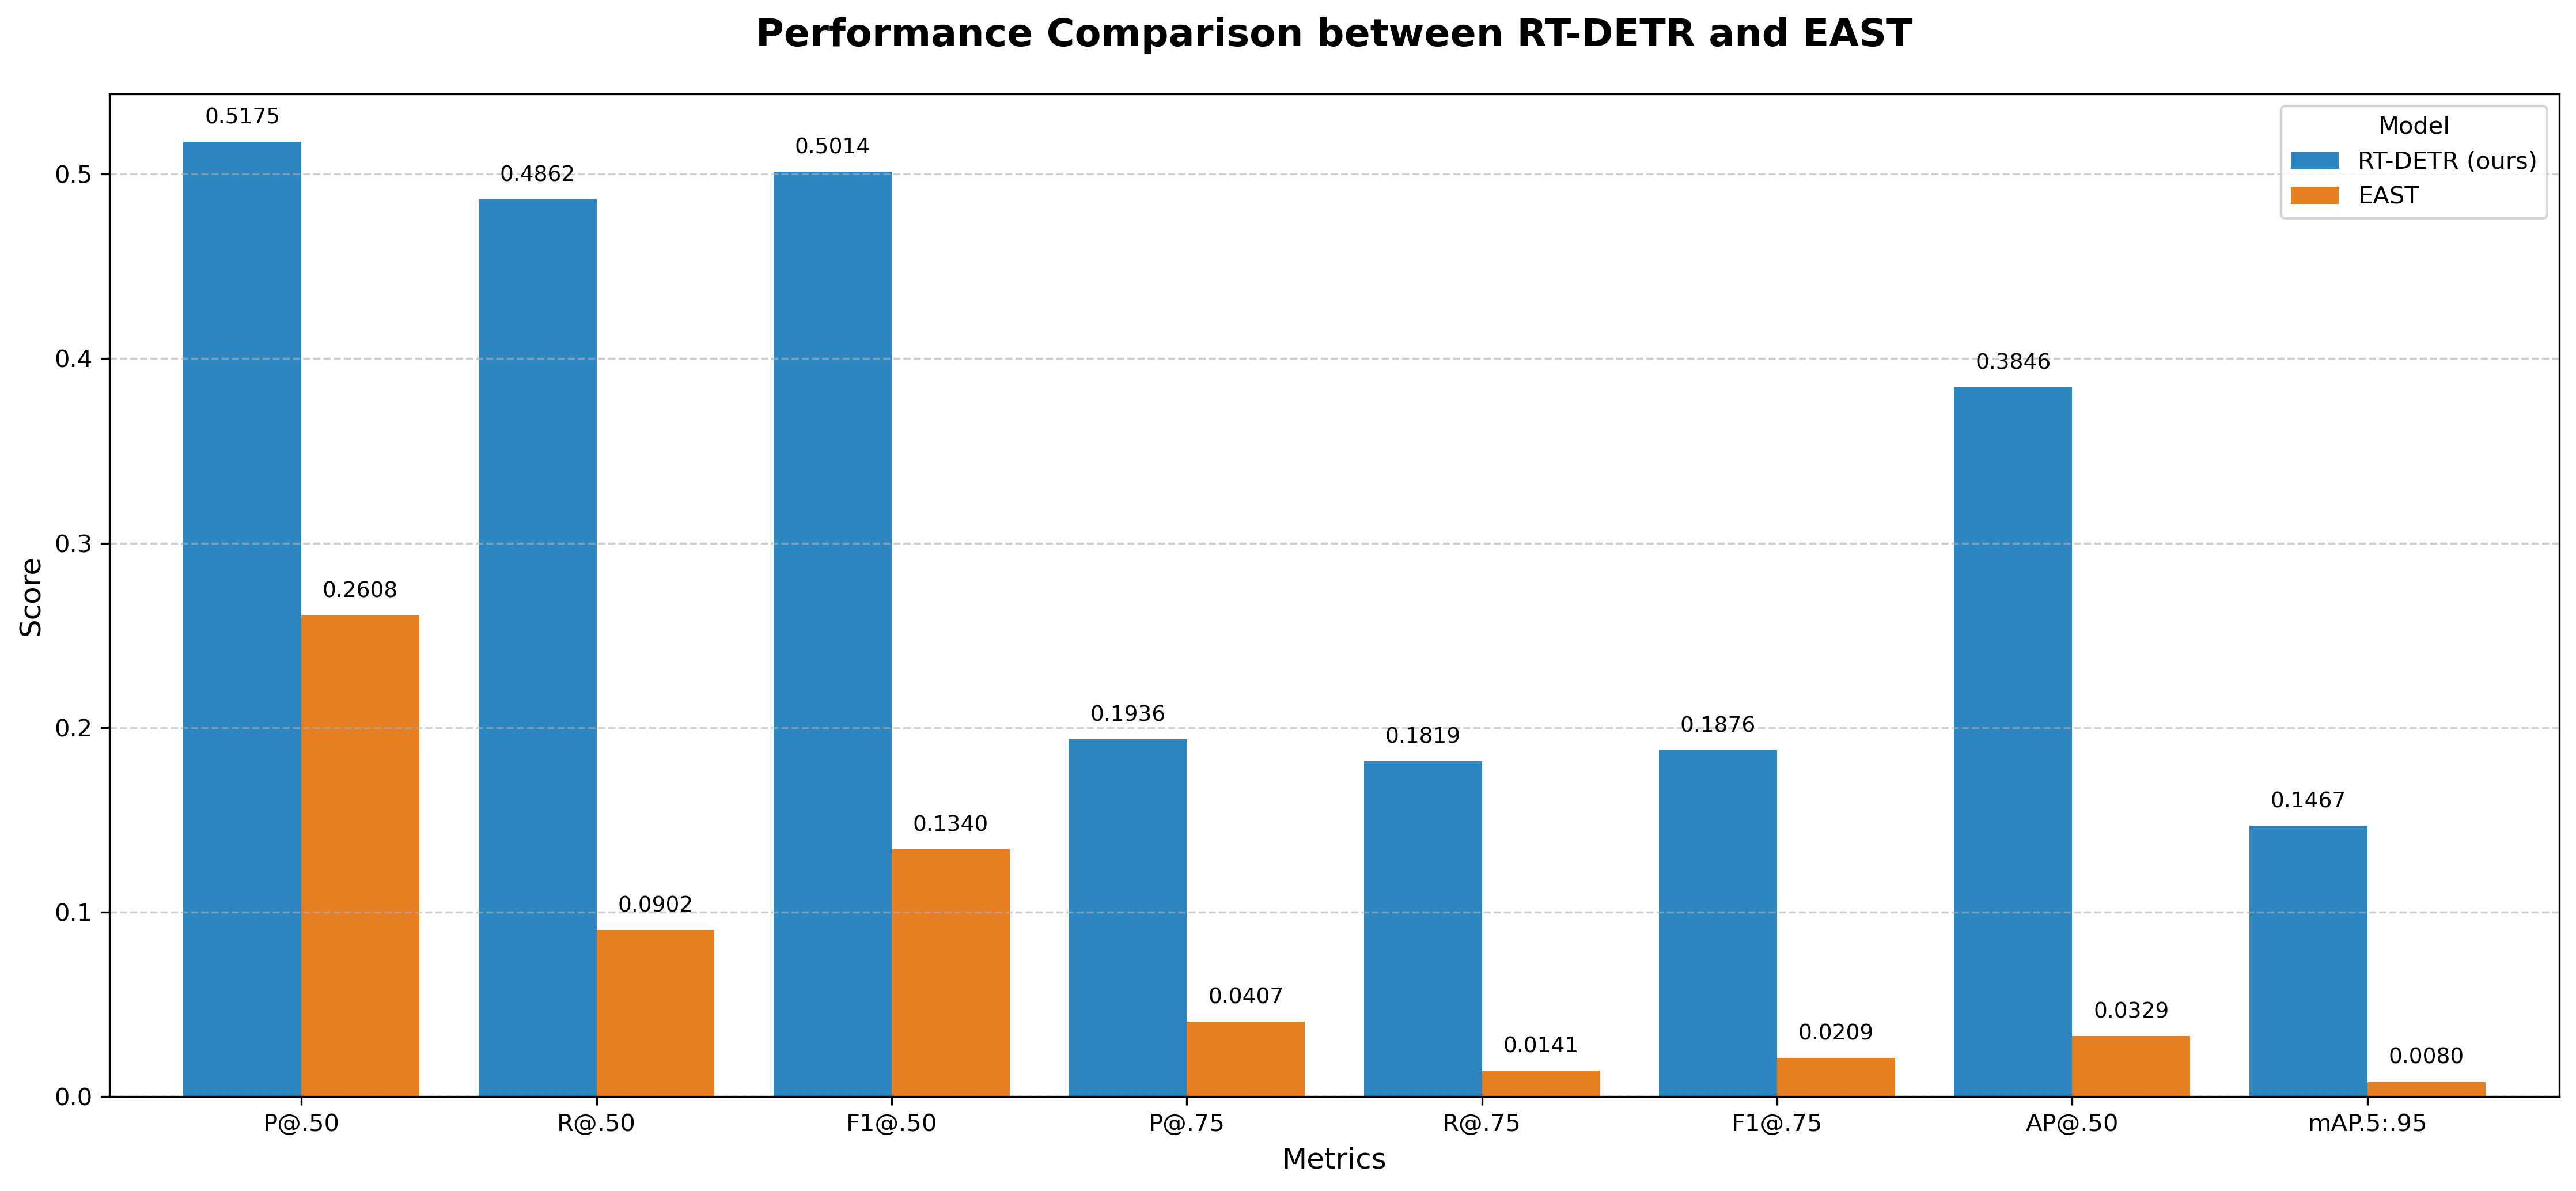
\includegraphics[width=\textwidth]{images/detection_bar_chart.png}
    \caption[Performance comparison between RT-DETR and EAST across detection metrics]{\textit{Performance comparison between RT-DETR and EAST across detection metrics.}}
    \label{fig:detection_bar}
\end{figure}

RT-DETR (blue) consistently outperforms EAST (orange) at both IoU thresholds of 0.50 and 0.75, with the gap widening substantially at the stricter threshold, reflecting the advantage of oriented bounding box regression. At IoU 0.50, RT-DETR leads across all three primary metrics: Precision (0.518 vs.\ 0.261), Recall (0.486 vs.\ 0.090), and F1-score (0.501 vs.\ 0.134), demonstrating that the fine-tuned model is both more accurate and more complete in its detections. The disparity becomes dramatically more pronounced at IoU 0.75: EAST's F1 collapses to 0.021 while RT-DETR retains an F1 of 0.188, a nearly tenfold difference. This behavior is consistent with the fundamental limitation of axis-aligned detectors on rotated text: EAST's horizontally constrained boxes may partially overlap a tilted text line at a loose threshold, but fail to achieve sufficient overlap under stricter criteria. The mAP across IoU thresholds from 0.50 to 0.95 (0.147 vs.\ 0.008) further encapsulates this localization quality gap in a single summary statistic.

A closer examination of the Precision and Recall figures at IoU 0.50 reveals an important asymmetry in how the two models fail. EAST achieves a Precision of 0.261, which is non-trivial in absolute terms, yet its Recall drops sharply to 0.090. This pattern indicates that while a portion of EAST's detections are positioned correctly enough to register as true positives at the lenient 0.50 threshold, the model misses a large fraction of text lines entirely. This systematic under-recall is attributable to two compounding factors. First, Vietnamese commercial documents such as receipts and invoices frequently contain text lines printed at slight angles or arranged in non-standard reading orders, layouts that fall outside the distribution of horizontal, left-to-right text that EAST was originally trained on. Second, EAST relies on a score map and geometry map predicted from a convolutional feature extractor, a pipeline that is highly sensitive to the scale and aspect ratio of text instances. When text lines are short, closely spaced, or partially occluded by document folds and scanning artifacts, the score map fails to produce confident activations, and the geometry map produces inaccurate offsets, both of which depress recall.

RT-DETR's architecture addresses these failure modes more directly. As a transformer-based detection framework, RT-DETR encodes global context through multi-head self-attention, which allows the model to attend to long-range relationships between distant text elements and to reason about document structure at the page level rather than locally. This global receptive field is particularly beneficial for Vietnamese documents, where the spatial arrangement of text lines often encodes semantic groupings (item descriptions versus prices, headers versus body text) that provide strong contextual cues for determining whether a candidate region contains a complete text line. In addition, the integration of the Gaussian Wasserstein Distance (GWD) loss directly supervises the angular parameter of oriented bounding boxes during training, providing a smooth and stable gradient signal even when the predicted angle differs substantially from the ground truth. By contrast, EAST's original quadrilateral regression loss does not explicitly enforce angular coherence, which leads to inconsistent angle predictions on oblique text.

The Precision value of 0.518 achieved by RT-DETR at IoU 0.50 also merits discussion. Although this figure may appear moderate in the context of object detection benchmarks on natural images, it reflects the inherent difficulty of the evaluation set rather than a weakness of the model per se. Vietnamese receipt documents exhibit high text density, with multiple short text lines printed in close proximity, and the ground truth annotations were generated using a strict line-level segmentation protocol in which individual text lines are annotated as separate instances even when they share a common baseline. Under this annotation scheme, a detection that spans two adjacent text lines is counted as a false positive even if it correctly localizes the text content, which artificially depresses Precision for any model that produces slightly oversized boxes. The AP@0.50 of 0.385 provides a more robust summary of precision-recall trade-offs, as it aggregates performance across all operating confidence thresholds and is less sensitive to the choice of a specific decision boundary.

The mAP@0.5:0.95 metric deserves particular attention because it integrates performance across eleven IoU thresholds from 0.50 to 0.95 in increments of 0.05, providing the most comprehensive single-number summary of localization quality. RT-DETR's mAP of 0.147 compared to EAST's 0.008 represents an 18-fold absolute improvement. The steep decline from AP@0.50 (0.385) to mAP@0.5:0.95 (0.147) observed for RT-DETR is consistent with typical behavior on dense text detection tasks, where achieving very tight box overlap (IoU above 0.85 or 0.90) requires the model to precisely align the predicted boundary with the outermost ink pixels of the text line. Even small errors in angle prediction or boundary placement accumulate significantly at these strict thresholds. Nonetheless, the fact that RT-DETR maintains a non-trivial mAP at the 0.5:0.95 range while EAST's mAP is effectively negligible (0.008) confirms that the oriented bounding box representation combined with GWD loss produces geometrically accurate predictions, not merely approximate localizations that happen to satisfy a lenient overlap criterion.

A qualitative illustration of this performance difference is provided in Figure~\ref{fig:qualitative_comparison}, which compares the detection outputs of both models on a representative sample Vietnamese receipt. As seen in the figure, RT-DETR provides much tighter bounding boxes that accurately adapt to the orientation of the text lines, whereas EAST produces loose, axis-aligned boxes that often fail to encompass the full extent of rotated text.

\begin{figure}[htbp]
    \centering
    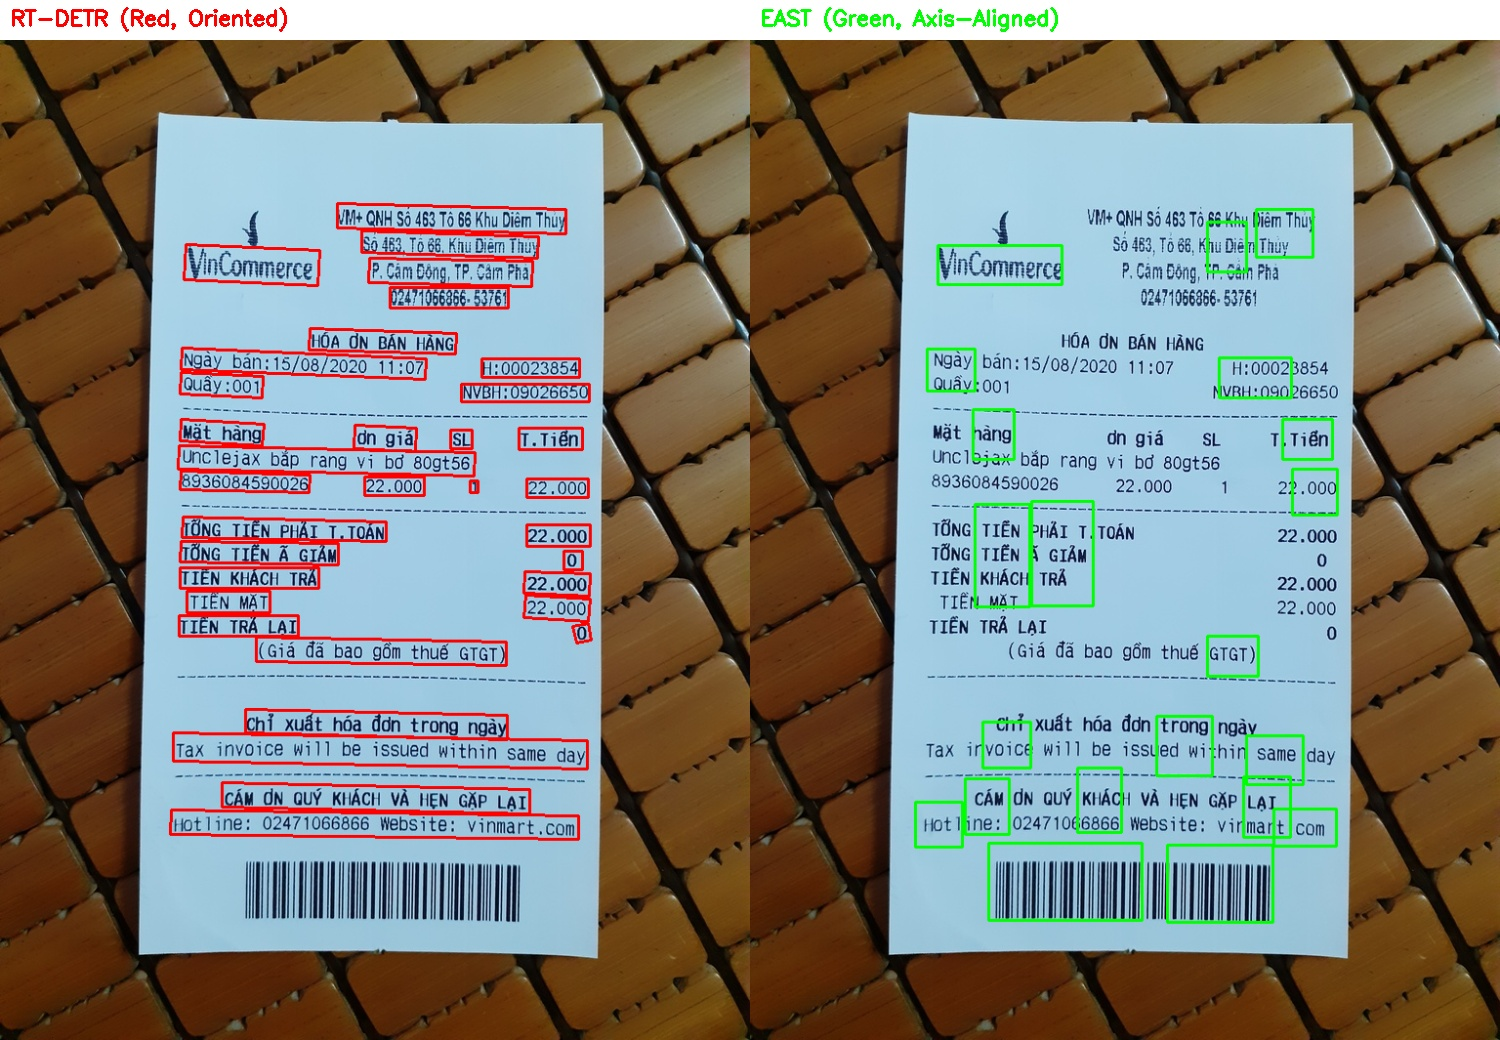
\includegraphics[width=0.6\linewidth]{images/detect_comparison.jpg}
    \caption[Qualitative comparison of text line detection between RT-DETR and EAST]{\textit{Qualitative comparison of text line detection between RT-DETR and EAST.}}
    \label{fig:qualitative_comparison}
\end{figure}

The proposed RT-DETR model (left, red oriented bounding boxes) produces tight detections that accurately conform to the orientation of the text lines. In contrast, the EAST baseline (right, green axis-aligned bounding boxes) produces loose, horizontally constrained boxes that frequently fail to encompass the full extent of rotated or skewed text, consistent with the large quantitative gap observed at higher IoU thresholds.

It is also worth noting that the absolute performance values of RT-DETR, while representing a clear state-of-the-art result on this specific benchmark, leave substantial room for future improvement. The F1 of 0.501 at IoU 0.50 indicates that roughly half of the predictions made by the model do not satisfy even the lenient overlap criterion, which has direct implications for the downstream recognition stage: any text line that is missed or poorly localized at detection time cannot be recovered by the recognizer regardless of its accuracy. Future work could address this limitation through several complementary strategies. Augmenting the training data with more diverse examples of extreme document degradation, heavy fold artifacts, and low-contrast printing conditions would improve the model's robustness to the tail of the document quality distribution. Additionally, incorporating document-level layout analysis as a pre-processing or auxiliary supervision step could help the detector distinguish between closely spaced text lines that the current model tends to merge into a single oversized prediction.

\subsection{Recognition Results}

Table~\ref{tab:recognition_results} reports Character Error Rate (CER) and Word Error Rate (WER) for the fine-tuned PARSeq model and the four baseline systems on the Vietnamese text line test set, where lower values indicate better performance.

\begin{table}[H]
\centering
\small
\caption[Text line recognition results on the Vietnamese test set]{\textit{Text line recognition results on the Vietnamese test set.}}
\label{tab:recognition_results}
\begin{tabular}{lcc}
\hline
\textbf{Model} & \textbf{CER (\%)} $\downarrow$ & \textbf{WER (\%)} $\downarrow$ \\
\hline
\textbf{PARSeq (ours)} & \textbf{10.18} & \textbf{34.71} \\
VietOCR & 11.34 & 37.44 \\
PaddleOCR & 16.79 & 62.40 \\
Tesseract & 20.61 & 56.68 \\
EasyOCR & 36.71 & 78.35 \\
\hline
\end{tabular}
\end{table}

The fine-tuned PARSeq model achieves the lowest CER of \textbf{10.18\%} and WER of \textbf{34.71\%} among all evaluated systems, outperforming the most competitive baseline VietOCR by 1.16 percentage points in CER and 2.73 percentage points in WER. The margin over general-purpose systems is substantially larger: PaddleOCR achieves a CER of \textbf{16.79\%} and WER of \textbf{62.40\%}, while EasyOCR produces the weakest results with a CER of \textbf{36.71\%} and WER of \textbf{78.35\%}, reflecting its limited adaptation to the morphological complexity of Vietnamese diacritical text. Tesseract, despite being a mature OCR engine with Vietnamese language support, achieves a CER of \textbf{20.61\%} and WER of \textbf{56.68\%}, indicating that its classical feature-based pipeline struggles with the full range of Vietnamese composite characters and font diversity present in the test set.

The WER values across all systems are notably higher than CER values, which is expected given the diacritical density of Vietnamese text: a single character error in a diacritically annotated word renders the entire word incorrect under WER. The absolute WER of \textbf{34.71\%} for PARSeq reflects the difficulty of the Vietnamese recognition task and indicates that there remains substantial room for improvement, particularly on rare tone-diacritic combinations and degraded image conditions.

These results confirm that domain-specific fine-tuning of PARSeq on Vietnamese synthetic data produces a model that surpasses all evaluated baselines, including VietOCR, which was specifically designed for Vietnamese text. The advantage of PARSeq over VietOCR is modest in CER terms but more pronounced in WER, suggesting that PARSeq's permutation-based bidirectional decoder provides consistent advantages in resolving whole-word diacritical ambiguities relative to unidirectional recognizers. Analysis of residual errors suggests that the majority of remaining mistakes occur on visually similar character pairs such as \textit{o}/\textit{ô}, \textit{a}/\textit{ă}, and \textit{u}/\textit{ư}, where the distinguishing diacritical mark occupies only a few pixels in the rendered image.

Figure~\ref{fig:recognition_bar} visualizes the CER and WER of all five evaluated models side by side, providing an at-a-glance comparison of their relative recognition quality on the Vietnamese test set.

\begin{figure}[htbp]
    \centering
    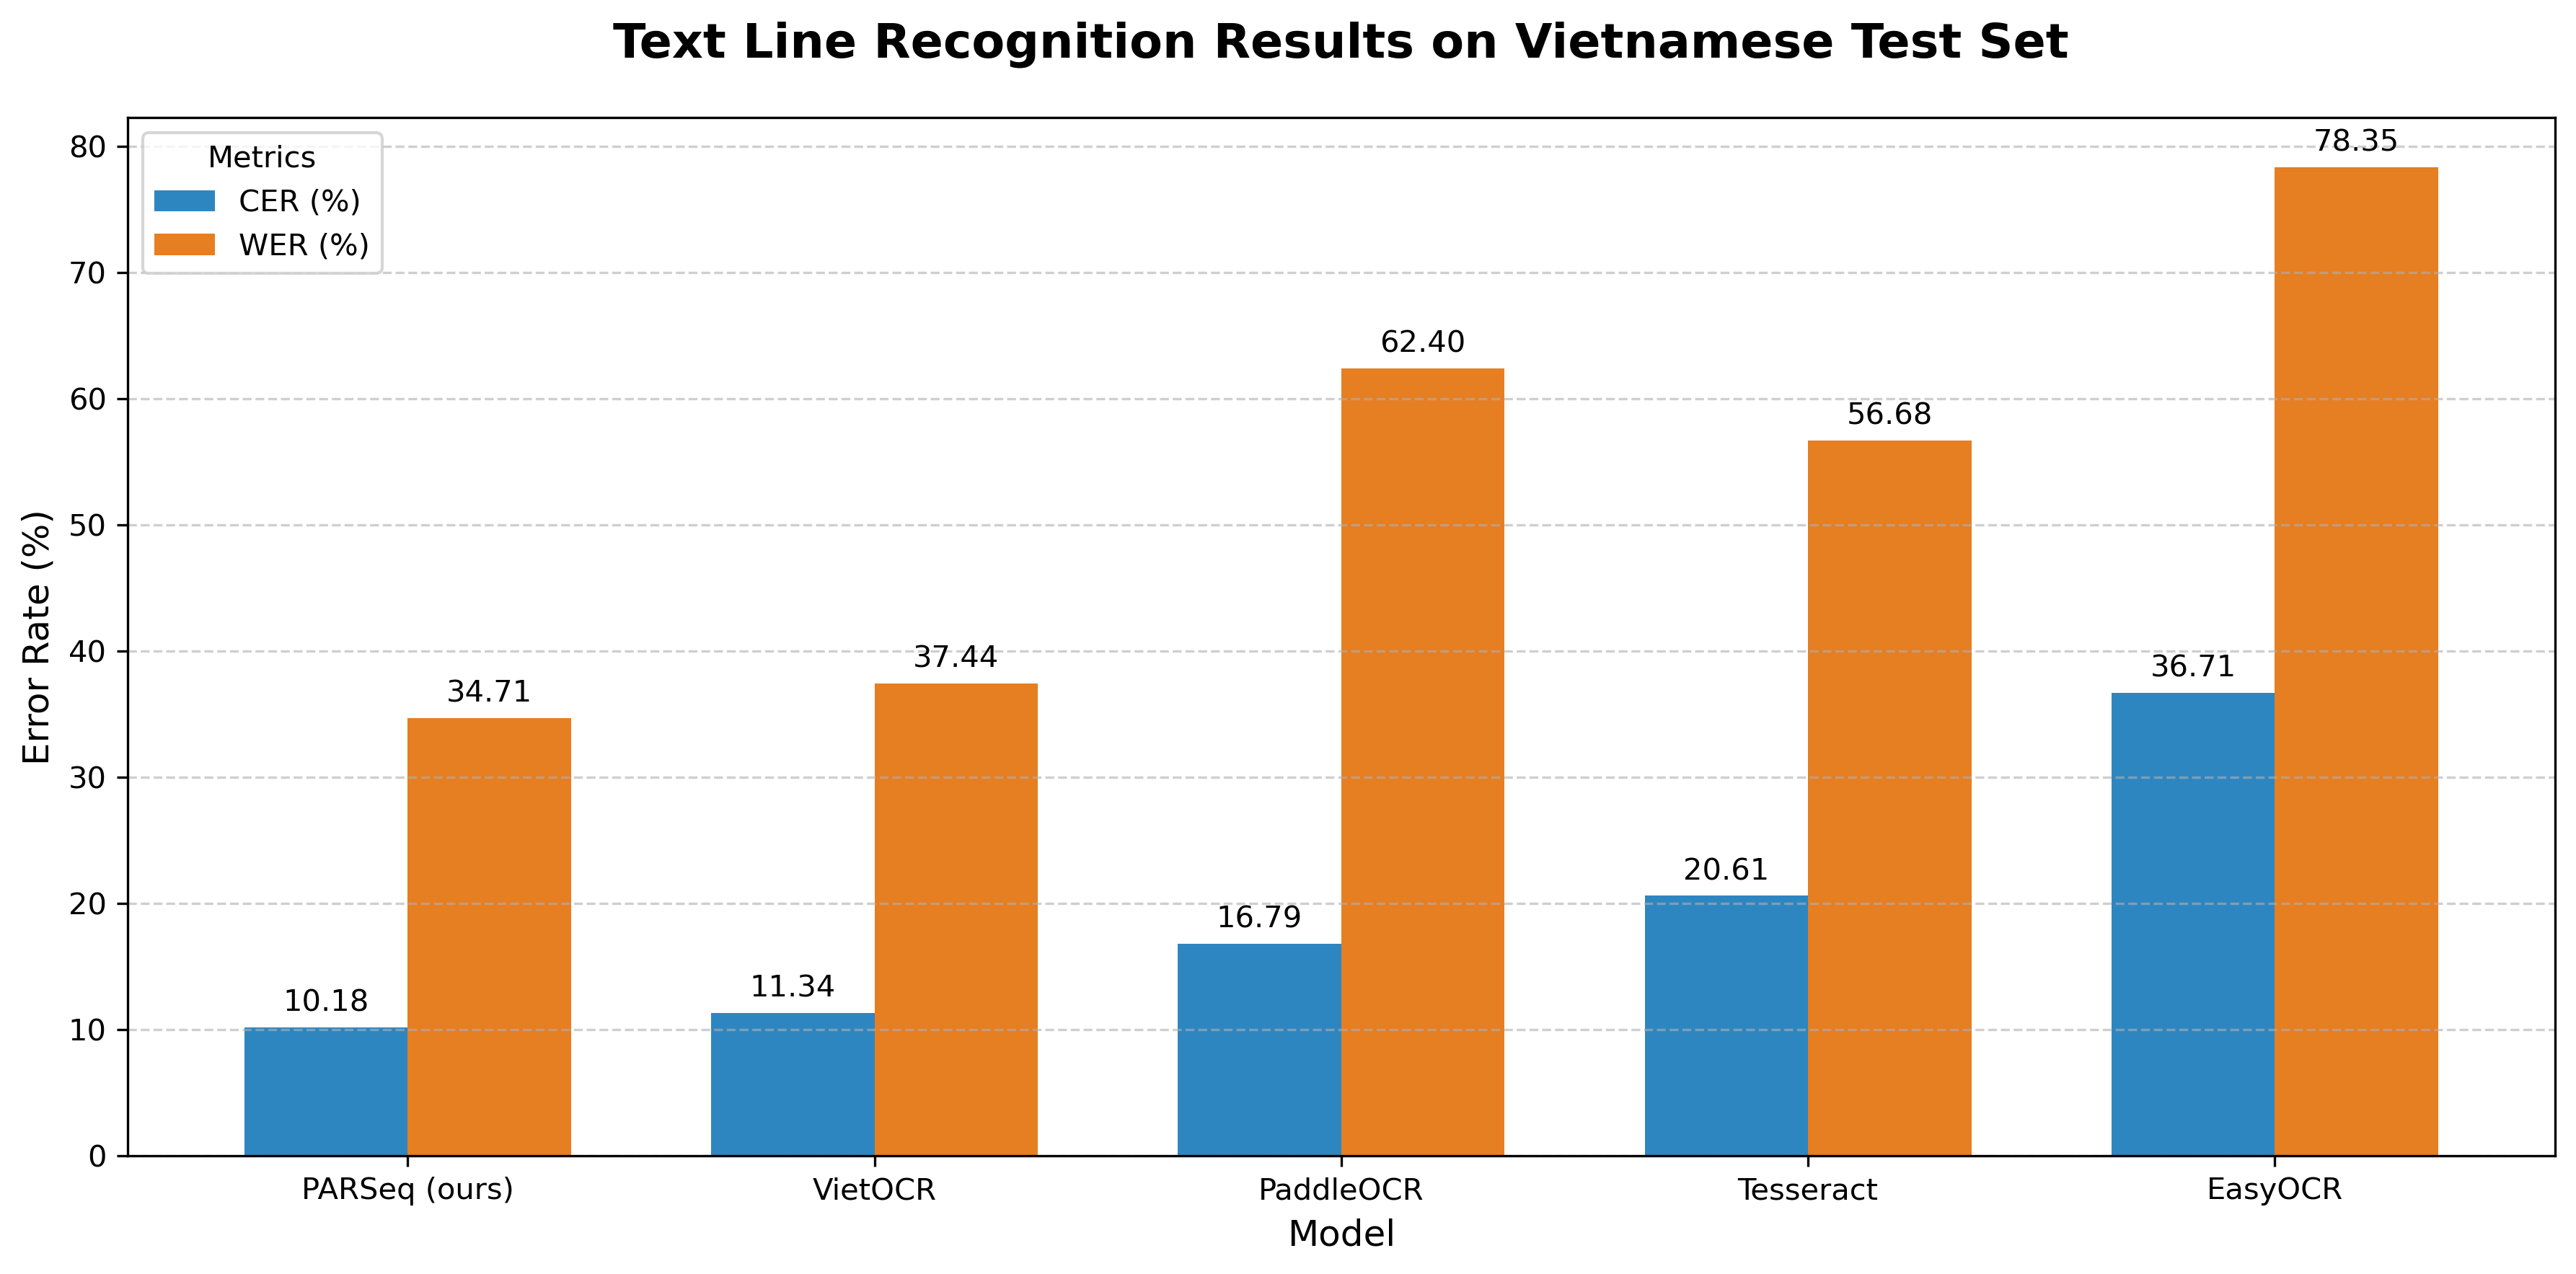
\includegraphics[width=\textwidth]{images/recognition_bar_chart.png}
    \caption[Text line recognition results on the Vietnamese test set]{\textit{Text line recognition results on the Vietnamese test set.}}
    \label{fig:recognition_bar}
\end{figure}

The chart makes two structural patterns immediately apparent. First, there is a clear performance tier: PARSeq and VietOCR form a top cluster with CER values below 12\%, while PaddleOCR, Tesseract, and EasyOCR occupy progressively worse positions with CER values ranging from 16.79\% to 36.71\%. Second, the WER consistently exceeds the corresponding CER for every model, a systematic effect attributable to the diacritical density of Vietnamese, where a single misrecognized tone mark invalidates an entire word under WER. This amplification is especially pronounced for EasyOCR (CER 36.71\% $\rightarrow$ WER 78.35\%) and PaddleOCR (CER 16.79\% $\rightarrow$ WER 62.40\%), indicating that these systems not only make more character-level errors but also tend to corrupt whole words rather than isolated characters. In contrast, PARSeq exhibits the smallest CER-to-WER ratio among all systems, suggesting that its permutation-based decoder produces errors that are more localized within words, a property that is practically valuable when downstream tasks depend on word-level extraction accuracy.

A deeper analysis of each model's error characteristics provides additional insight into why the performance tiers emerge as they do. The PARSeq architecture is particularly well-suited to the Vietnamese recognition task for several interconnected reasons. Unlike conventional unidirectional sequential decoders that predict characters from left to right, PARSeq employs a permutation language model during training that exposes the decoder to all possible orderings of the output sequence. This means that at inference time, the model's predictions for each character position are implicitly conditioned on both the left and right context, even when decoding autoregressively. For Vietnamese, where the disambiguation of a vowel base character (e.g., distinguishing \textit{a}, \textit{ă}, and \textit{â}) depends on a combination of tone mark and vowel modification diacritic that may span adjacent character positions in the rendered image, bidirectional context provides a critical advantage. A model that has only seen the leftward context when predicting a diacritic has less information available to resolve ambiguous visual evidence than one that can simultaneously attend to neighboring character shapes.

VietOCR's competitive performance despite its unidirectional architecture can be attributed to the fact that it was pretrained specifically on Vietnamese text and therefore has a strong prior over the co-occurrence patterns of Vietnamese character sequences. The model's internal language model, implicitly encoded in its recurrent decoder weights, effectively compensates for the lack of explicit right-to-left context by assigning high probability to diacritic combinations that are linguistically valid in Vietnamese. However, this same language model prior becomes a liability when the test text contains domain-specific tokens such as product names, abbreviated units of measurement, or alphanumeric codes that appear frequently in receipt documents but infrequently in the natural language text on which VietOCR was fine-tuned. In these cases, the unidirectional decoder's tendency to complete familiar morphological patterns can override the visual evidence and produce lexically plausible but contextually incorrect predictions.

PaddleOCR's performance is substantially worse, with a CER of 16.79\% representing a degradation of more than 6 percentage points relative to VietOCR. This gap is largely attributable to the fact that PaddleOCR, in its default multilingual configuration, distributes its model capacity across a large number of scripts and languages. The Vietnamese character set, which includes 134 distinct letter-diacritic combinations across six tone categories, requires a recognition model with sufficient representational capacity dedicated to resolving fine-grained visual distinctions within the Latin extended range. A model that must simultaneously handle Arabic, Chinese, Thai, and dozens of other scripts has inherently less capacity available per script, and the resulting feature representations for Vietnamese diacritics are less discriminative than those of a model trained exclusively or primarily on Vietnamese. Additionally, PaddleOCR's text normalization pipeline may apply Unicode normalization procedures that inadvertently merge distinct Vietnamese precomposed characters with visually similar but semantically different decomposed forms, introducing systematic substitution errors that inflate both CER and WER independently of the visual recognition quality.

Tesseract's CER of 20.61\% and WER of 56.68\% reflect the fundamental architectural mismatch between its classical pattern-recognition pipeline and the requirements of modern Vietnamese document OCR. Tesseract's recognition engine was originally designed around a set of hand-crafted feature extractors optimized for Latin typefaces, and while the addition of an LSTM layer in version 4 improved its handling of cursive and variable-width scripts, the system remains heavily dependent on its internal character segmentation module. For Vietnamese, where multiple combining diacritics may be stacked vertically above or below a base character, the segmentation module frequently produces incorrect cut points that either merge two characters into a single segment or split a single composite character into multiple fragments. These segmentation errors propagate to the recognition stage as either substitution errors (when a merged segment is misidentified as a different character) or insertion/deletion errors (when a fragmented segment produces extra or missing output tokens), both of which are counted in CER and amplified in WER.

EasyOCR produces the worst results across both metrics, with a CER of 36.71\% and WER of 78.35\%. These figures indicate that EasyOCR's recognition model fails on a majority of Vietnamese words present in the test set, which is consistent with its design as a lightweight, broadly multilingual system. EasyOCR's Vietnamese support was added through the inclusion of a small Vietnamese-specific recognition head trained on a relatively limited synthetic corpus, without the extensive domain-specific fine-tuning that characterizes both PARSeq and VietOCR. As a result, the model is highly sensitive to font diversity, performing reasonably on common sans-serif typefaces but degrading severely on the condensed, bold, and decorative fonts that are prevalent in Vietnamese retail receipts and commercial documents. The particularly large WER of 78.35\% compared to CER of 36.71\% also suggests that EasyOCR's errors are not uniformly distributed across character positions but tend to cluster at diacritical positions within words, which disproportionately invalidates entire word predictions under the WER metric.

The ratio between WER and CER across all models also serves as an informative diagnostic signal. For a language with uniformly distributed character errors and words of average length $L$, the expected WER given a CER of $\epsilon$ is approximately $1 - (1 - \epsilon)^L$. Vietnamese words have an average length of approximately 2 to 3 characters (using the syllable as the basic orthographic unit), which would predict a WER of roughly 19\% to 27\% for a CER of 10\%, assuming uniformly distributed errors. The observed WER of 34.71\% for PARSeq is higher than this theoretical expectation, indicating that errors are not uniformly distributed but are concentrated at the diacritical characters that appear in most Vietnamese syllables. This non-uniform error distribution is consistent with the residual error analysis reported above and confirms that diacritic resolution remains the primary bottleneck for Vietnamese OCR performance regardless of the overall architectural approach.

To provide further insight into these quantitative metrics and the specific challenges of Vietnamese diacritics, Figure~\ref{fig:recognition_qualitative} presents a qualitative comparison of the recognition outputs across the evaluated models. As shown, the fine-tuned PARSeq model is highly robust to varying image conditions and complex tone marks, whereas the baseline systems frequently fail to capture the correct diacritics or substitute characters entirely.

\begin{figure}[htbp]
    \centering
    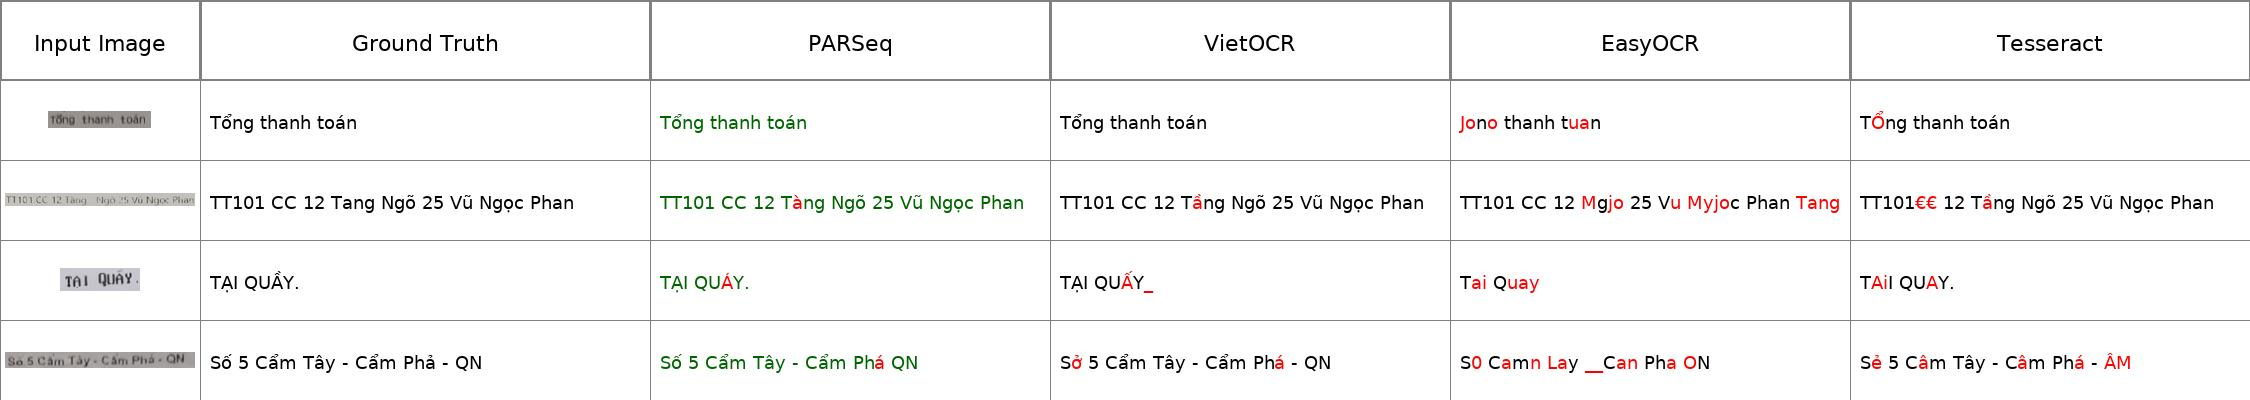
\includegraphics[width=\textwidth]{images/recog_comparison.jpg}
    \caption[Qualitative comparison of text recognition results across different models]{\textit{Qualitative comparison of text recognition results across different models.}}
    \label{fig:recognition_qualitative}
\end{figure}

The fine-tuned PARSeq model demonstrates strong robustness to varying image conditions and complex tone marks, correctly resolving diacritical combinations that other systems fail to handle (correct predictions highlighted in green). In contrast, baseline models exhibit characteristic failure modes: VietOCR occasionally misidentifies vowel modification diacritics under low-resolution conditions; EasyOCR produces frequent character substitutions and drops tonal markers entirely on degraded inputs; and Tesseract inserts spurious symbols and fails to recognize composite Vietnamese glyphs, reflecting its lack of native Vietnamese diacritical support. These qualitative observations are consistent with the CER and WER differences reported in Table~\ref{tab:recognition_results} and illustrate concretely why diacritical accuracy is critical for Vietnamese OCR in practical deployment.

From an end-to-end system perspective, it is important to consider the joint effect of detection and recognition errors on the overall pipeline's utility. A text line that is correctly detected but incorrectly recognized contributes to WER at the recognition stage, whereas a text line that is missed at detection contributes an implicit 100\% word error for that line (since no recognition output is produced). Given that RT-DETR achieves a Recall of 0.486 at IoU 0.50, approximately half of the text lines in the evaluation set produce no recognition output at all, which means the effective end-to-end WER is substantially higher than the isolated recognition WER of 34.71\% reported in Table~\ref{tab:recognition_results}. This observation underscores that improving detection recall is at least as important as improving recognition accuracy for practical Vietnamese document processing, and that future work should prioritize detection coverage alongside recognition quality to achieve meaningful gains in downstream information extraction tasks.
